\documentclass[a4paper,11pt,stu]{apa}


% Set double spacing
\usepackage{setspace}

% Set captions
\usepackage[
    format=plain,
    font=normalsize,
    labelfont=bf,
    textfont=it,
    labelsep=newline]{caption}
\captionsetup{
    justification=raggedright,
    singlelinecheck=false,
    margin=0cm
    } % Align left
%\AtEveryCite{\normalfont} % Prevent italic anywhere else in the document
\usepackage[capposition=top]{floatrow} % For ``Note.'' underneath the figures
%\DeclareCaptionFont{normal}{\fontsize{11}{13.2}\selectfont}
%\newcommand{\fignote}[1]{\floatsetup{font=normal,cappositon=bottom}\floatfoot{\large \textit{Note.} #1}}

\usepackage{tikz}
\usetikzlibrary{automata,shapes,arrows,calc,positioning,decorations.pathmorphing}

\begin{document}

\begin{figure}[!h]
    \caption{Modelresultater}
    \label{fig:dk}

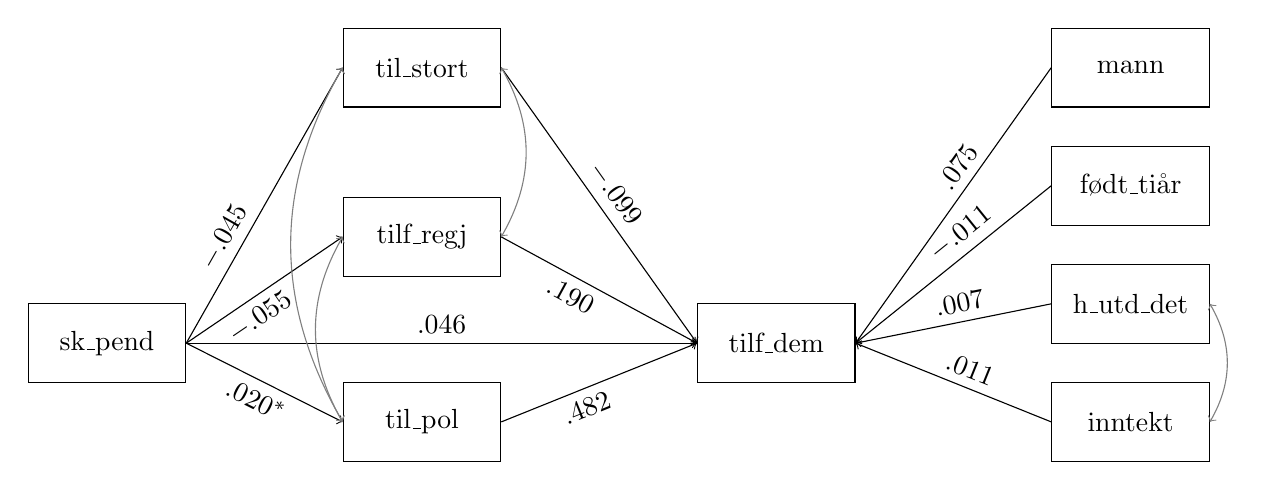
\begin{tikzpicture}[
    manvar/.style={rectangle,draw=black,minimum width=2cm,minimum height=1cm},
    convar/.style={rectangle,draw=black,minimum width=2cm,minimum height=1cm,fill=gray!50},
    vartype/.style={rectangle,draw=white,minimum width=2cm,minimum height=1cm},
    bend angle=-30,
    decoration={
        zigzag,
        amplitude=1pt,
        segment length=1mm,
        post=lineto,
        post length=4pt
    }
]

% Draw input variable (X)
    \node[manvar] (skd) at (0,0) {sk$\_$pend};

% Draw mediators (M)
    \node[manvar] (sto) at (4,3.5) {til$\_$stort};
    \node[manvar] (reg) at (4,1.35) {tilf$\_$regj};
    \node[manvar] (pol) at (4,-1) {til$\_$pol};

% Draw outcome variable (Y)
    \node[manvar] (dem) at (8.5,0) {tilf$\_$dem};

% Draw control variables (C)
    \node[manvar] (kjn) at (13,3.5) {mann};
    \node[manvar] (ald) at (13,2) {født$\_$tiår};
    \node[manvar] (utd) at (13,0.5) {h$\_$utd$\_$det};
    \node[manvar] (int) at (13,-1) {inntekt};

% Link X to M
    \draw[->] (skd.east) to node[above,sloped,pos=0.35] {$-.045$} (sto.west);
    \draw[->] (skd.east) to node[below,sloped,pos=0.4] {$-.055$} (reg.west);
    \draw[->] (skd.east) to node[below,sloped] {$.020^*$} (pol.west);
% Link M to Y
    \draw[->] (sto.east) to node[above,sloped] {$-.099$} (dem.west);
    \draw[->] (reg.east) to node[below,sloped,pos=.4] {$.190$} (dem.west);
    \draw[->] (pol.east) to node[below,sloped,pos=.4] {$.482$} (dem.west);
% Link X to Y
    \draw[->] (skd.east) to node[above] {$.046$} (dem.west);
% Link C to Y
    \draw[->] (kjn.west) to node[above,sloped,pos=0.4] {$.075$} (dem.east);
    \draw[->] (ald.west) to node[above,sloped,pos=0.4] {$-.011$} (dem.east);
    \draw[->] (utd.west) to node[above,sloped,pos=0.45] {$.007$} (dem.east);
    \draw[->] (int.west) to node[above,sloped,pos=0.45] {$.011$} (dem.east);

% Allow correlation between i and s
    \draw[<->,gray] (sto.east) to [bend right] (reg.east);
    \draw[<->,gray] (sto.west) to [bend left] (pol.west);
    \draw[<->,gray] (reg.west) to [bend left] (pol.west);
    \draw[<->,gray] (utd.east) to [bend right] (int.east);

% % Link T to d
%     \draw[dashed,->] (t1.south) to (d1.north);
%     \draw[dashed,->] (t2.south) to (d1.north);

%     \draw[dashed,->] (t2.south) to (d2.north);
%     \draw[dashed,->] (t3.south) to (d2.north);

\end{tikzpicture}

    \floatfoot{\normalsize \textit{Notis.}
    }
\end{figure}

\end{document}